%!TEX root = Bericht.tex
\chapter{Appendix}\label{cha:appendix}

\section{Parameterizations}
\subsection{Arc Length Distribution}
\label{subsec:arcLengthDistribution}
TO DO
\subsection{Effect of different Parameterizations with cubic, quartic and quintic splines}
\label{subsec:parameterization_degree}

\begin{figure}[H]
  \begin{minipage}[t]{0.9\textwidth}
    \includegraphics[width = \textwidth]{graphics/Parameterization345_road_agile.eps}
  \end{minipage}
  \caption{The different parameterizations shown with cubic, quartic and quintic splines}
  \label{fig:parameterization_cqq}
\end{figure}

\section{Trajectory Control Results}

\begin{figure}[h]
  \begin{minipage}[t]{0.32\textwidth}
    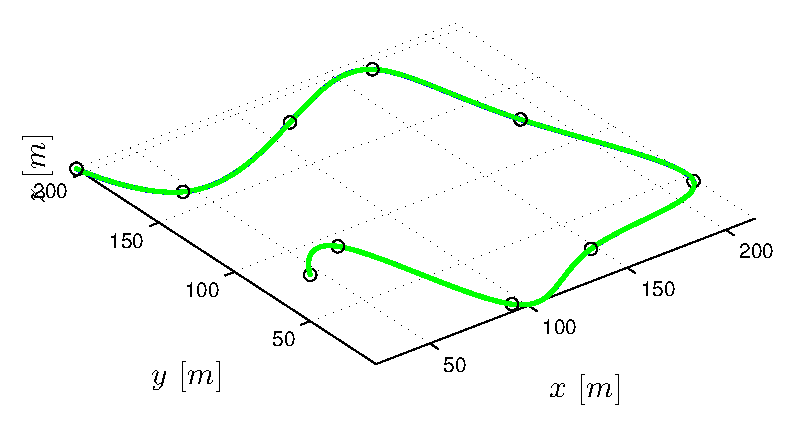
\includegraphics[width = \textwidth]{trackings/figure_3D_road_SplineDegree3_trajectoryFollowing_Disturbance_0}
  \end{minipage}
  \hfill
  \begin{minipage}[t]{0.32\textwidth}
    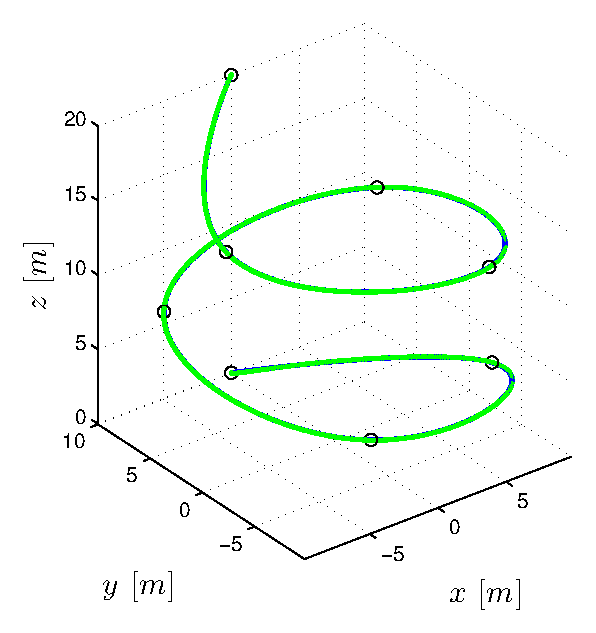
\includegraphics[width = \textwidth]{trackings/figure_3D_helix_SplineDegree3_trajectoryFollowing_Disturbance_0}
  \end{minipage}
  \hfill
  \begin{minipage}[t]{0.32\textwidth}
    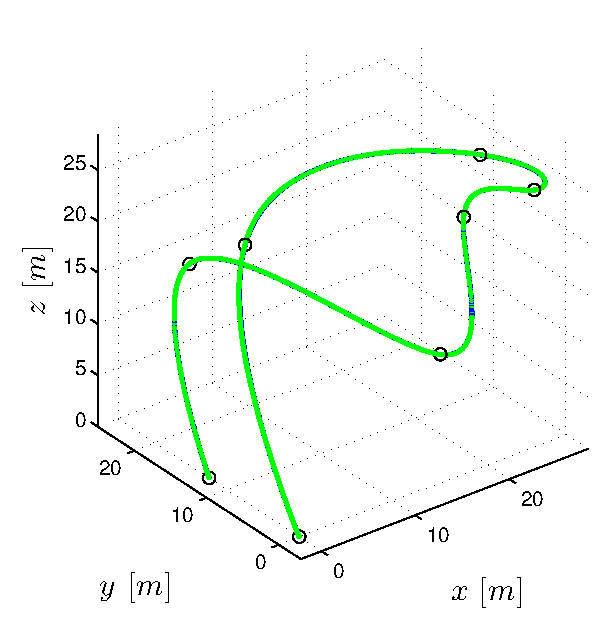
\includegraphics[width = \textwidth]{trackings/figure_3D_agile_SplineDegree3_trajectoryFollowing_Disturbance_0}
  \end{minipage}
  %\caption{BLA tracking }
  \vspace{5pt}
  \begin{minipage}[t]{0.32\textwidth}
    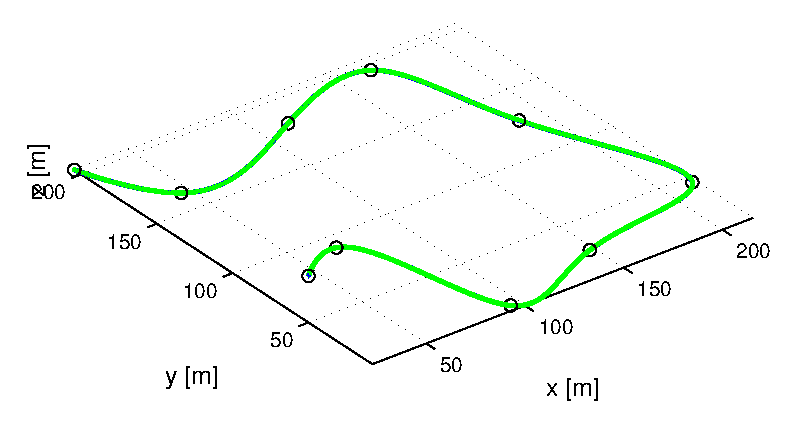
\includegraphics[width = \textwidth]{trackings/figure_3D_road_SplineDegree3_purePursuit_Disturbance_0}
  \end{minipage}
  \hfill
  \begin{minipage}[t]{0.32\textwidth}
    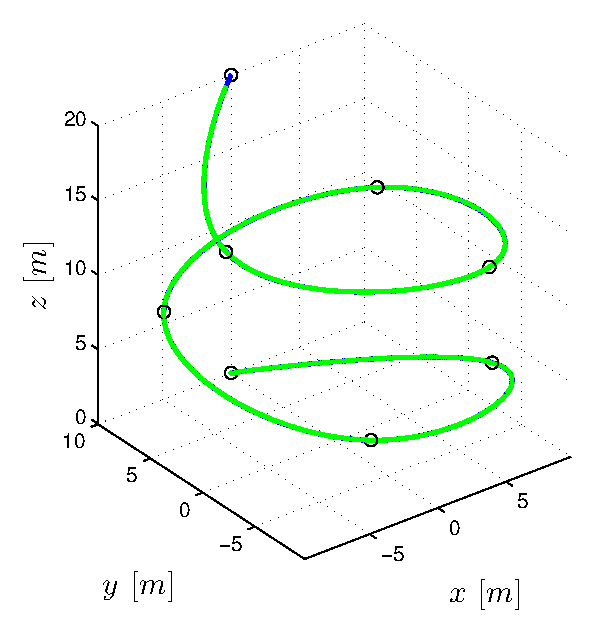
\includegraphics[width = \textwidth]{trackings/figure_3D_helix_SplineDegree3_purePursuit_Disturbance_0}
  \end{minipage}
  \hfill
  \begin{minipage}[t]{0.32\textwidth}
    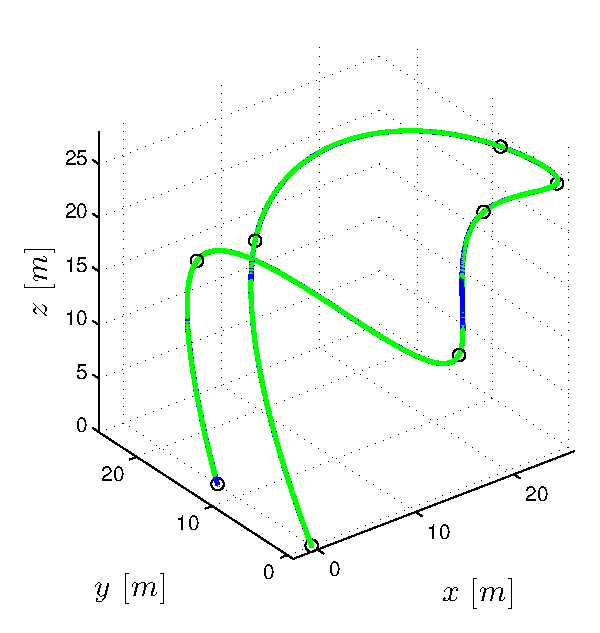
\includegraphics[width = \textwidth]{trackings/figure_3D_agile_SplineDegree3_purePursuit_Disturbance_0}
  \end{minipage}
  %\caption{BLA tracking }
  \vspace{5pt}
  \begin{minipage}[t]{0.32\textwidth}
    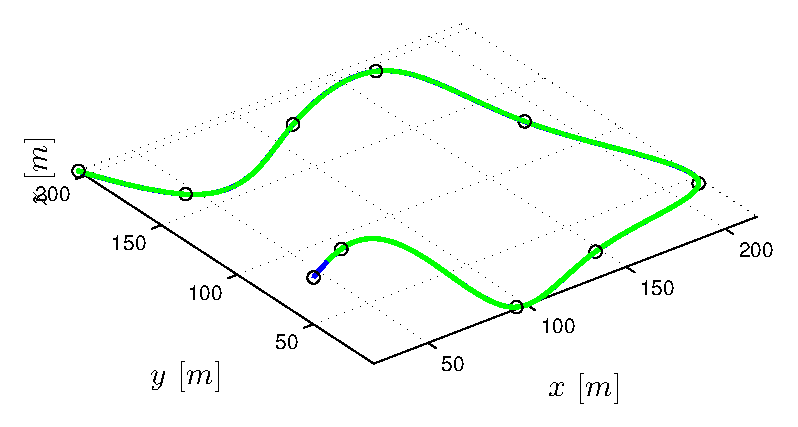
\includegraphics[width = \textwidth]{trackings/figure_3D_road_SplineDegree3_crossTrack_Disturbance_0}
  \end{minipage}
  \hfill
  \begin{minipage}[t]{0.32\textwidth}
    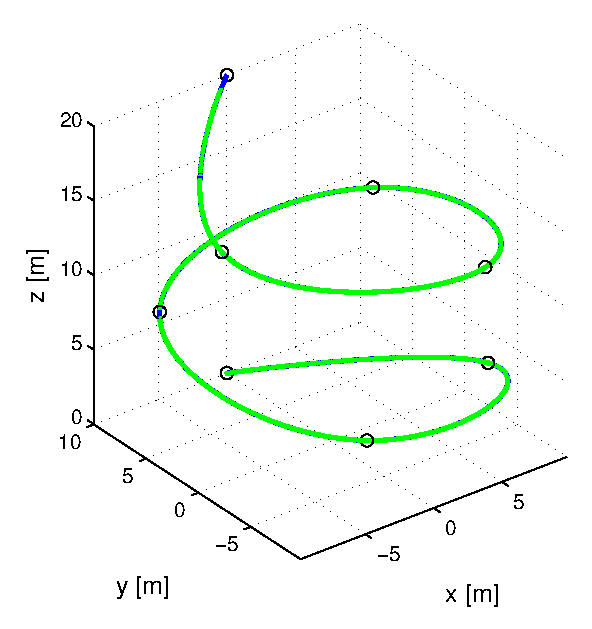
\includegraphics[width = \textwidth]{trackings/figure_3D_helix_SplineDegree3_crossTrack_Disturbance_0}
  \end{minipage}
  \hfill
  \begin{minipage}[t]{0.32\textwidth}
    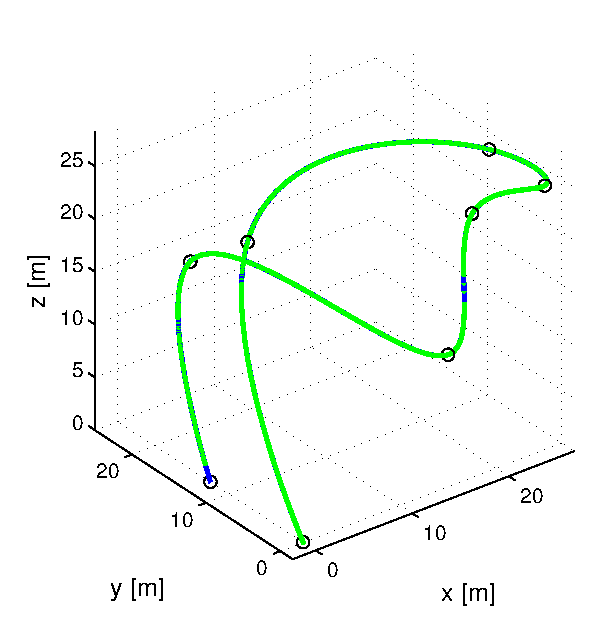
\includegraphics[width = \textwidth]{trackings/figure_3D_agile_SplineDegree3_crossTrack_Disturbance_0}
  \end{minipage}
  \caption{Trajectory tracking with perfect model estimation. {\bf Top}: \textit{Trajectory following} control {\bf Center}: \textit{Pure pursuit} control {\bf Bottom}: \textit{Cross track error} control}
  \label{fig:results_perfect_model}
\end{figure}

\begin{figure}[h]
  \begin{minipage}[t]{0.32\textwidth}
    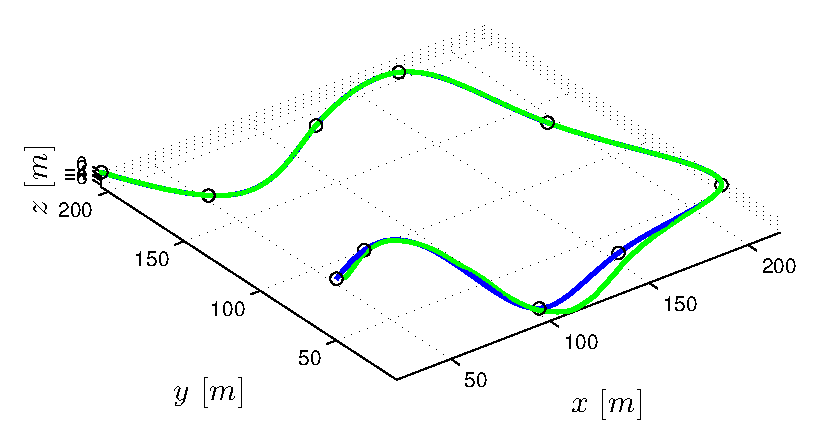
\includegraphics[width = \textwidth]{trackings/figure_3D_road_SplineDegree3_trajectoryFollowing_Disturbance_1}
  \end{minipage}
  \hfill
  \begin{minipage}[t]{0.32\textwidth}
    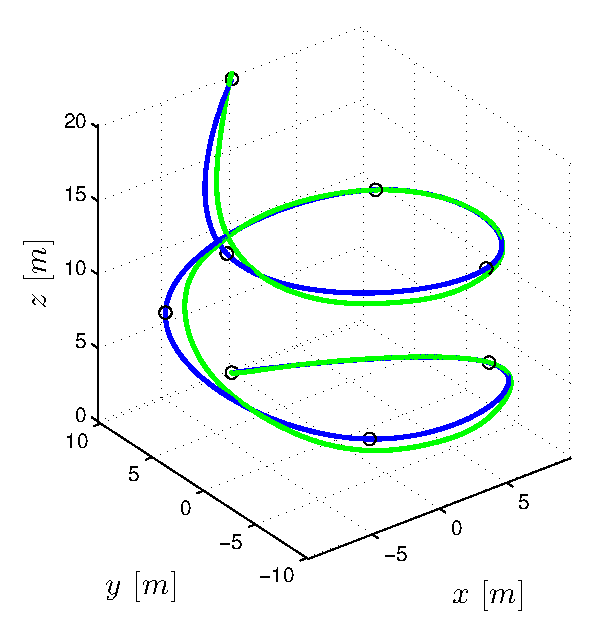
\includegraphics[width = \textwidth]{trackings/figure_3D_helix_SplineDegree3_trajectoryFollowing_Disturbance_1}
  \end{minipage}
  \hfill
  \begin{minipage}[t]{0.32\textwidth}
    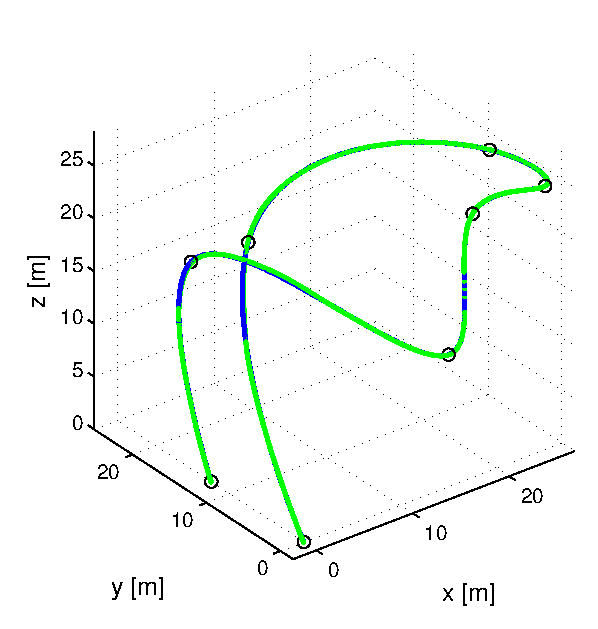
\includegraphics[width = \textwidth]{trackings/figure_3D_agile_SplineDegree3_trajectoryFollowing_Disturbance_1}
  \end{minipage}
  %\caption{BLA tracking }
  \vspace{5pt}
  \begin{minipage}[t]{0.32\textwidth}
    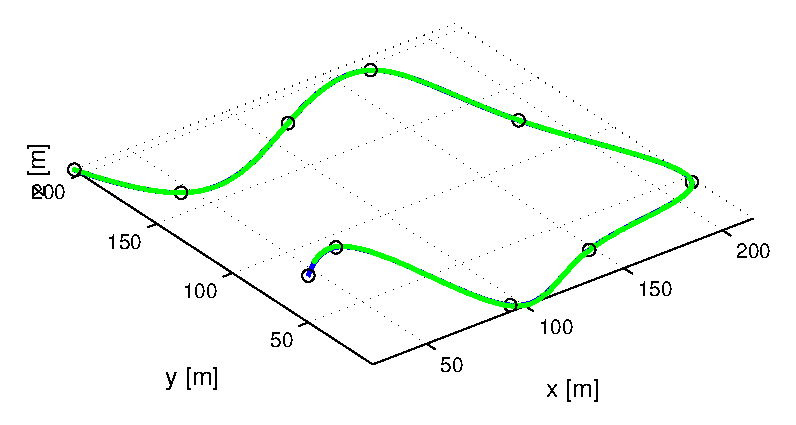
\includegraphics[width = \textwidth]{trackings/figure_3D_road_SplineDegree3_purePursuit_Disturbance_1}
  \end{minipage}
  \hfill
  \begin{minipage}[t]{0.32\textwidth}
    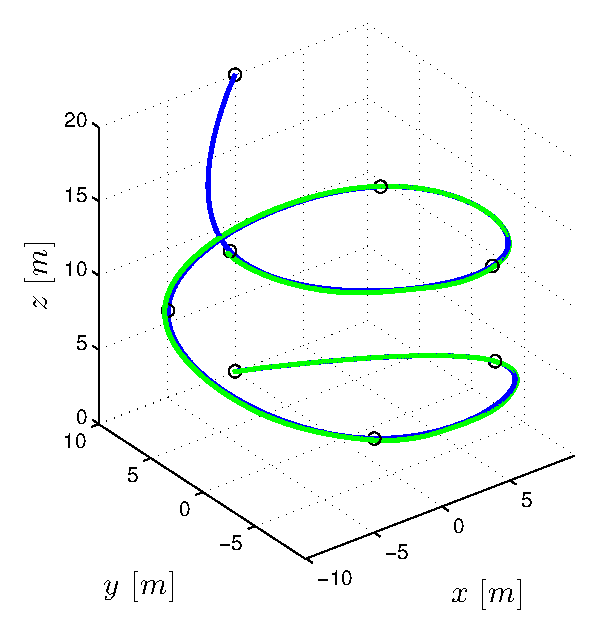
\includegraphics[width = \textwidth]{trackings/figure_3D_helix_SplineDegree3_purePursuit_Disturbance_1}
  \end{minipage}
  \hfill
  \begin{minipage}[t]{0.32\textwidth}
    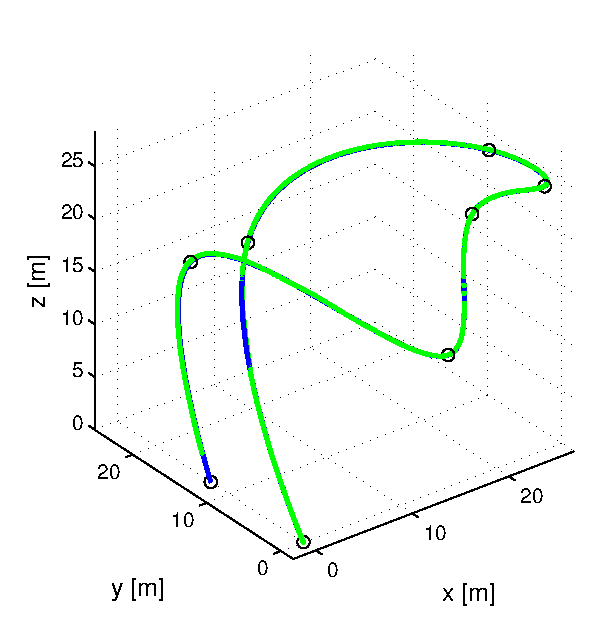
\includegraphics[width = \textwidth]{trackings/figure_3D_agile_SplineDegree3_purePursuit_Disturbance_1}
  \end{minipage}
  %\caption{BLA tracking }
  \vspace{5pt}
  \begin{minipage}[t]{0.32\textwidth}
    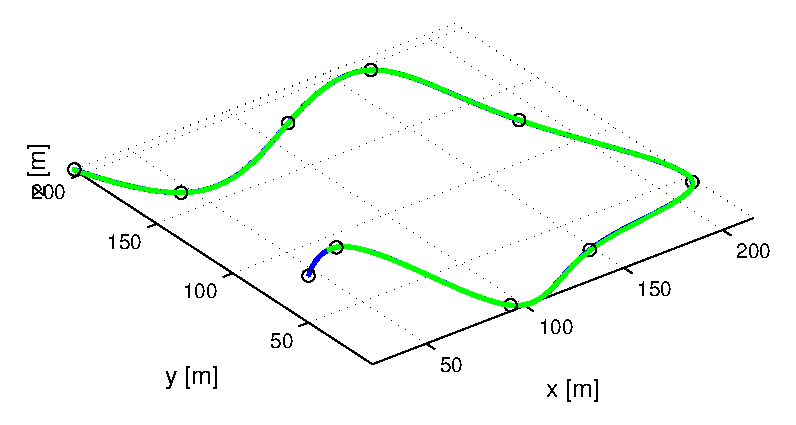
\includegraphics[width = \textwidth]{trackings/figure_3D_road_SplineDegree3_crossTrack_Disturbance_1}
  \end{minipage}
  \hfill
  \begin{minipage}[t]{0.32\textwidth}
    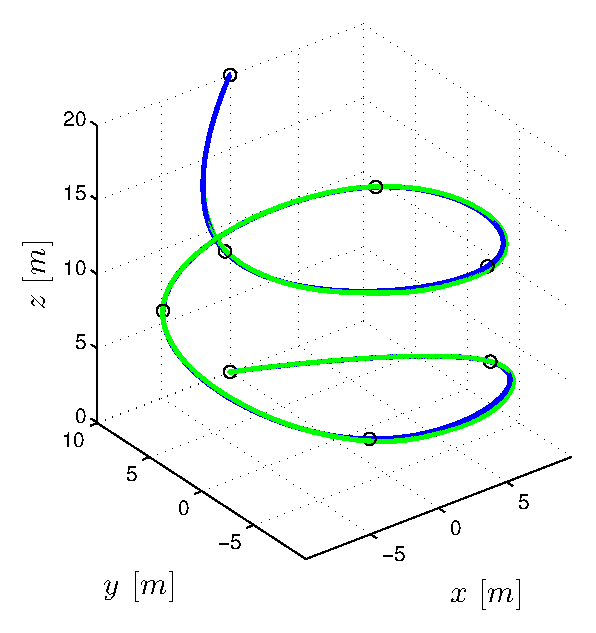
\includegraphics[width = \textwidth]{trackings/figure_3D_helix_SplineDegree3_crossTrack_Disturbance_1}
  \end{minipage}
  \hfill
  \begin{minipage}[t]{0.32\textwidth}
    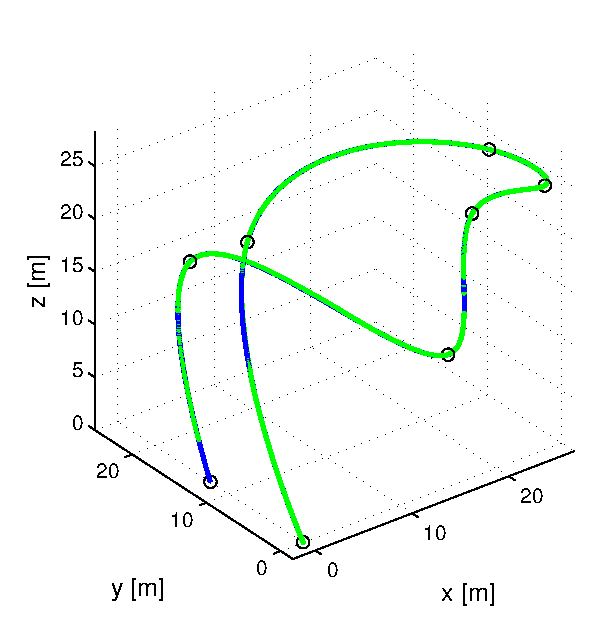
\includegraphics[width = \textwidth]{trackings/figure_3D_agile_SplineDegree3_crossTrack_Disturbance_1}
  \end{minipage}
  \caption{Trajectory tracking with wind disturbance (1~m/s x-direction). {\bf Top}: \textit{Trajectory following} control forces the system to reach the end within the given constraints. As trajectory constraints do not consider wind, tracking errors are high. {\bf Center}: \textit{Pure pursuit} control is more robust to wind and the tracking still accurate. In comparison to the ideal case it only makes only 85-95\% of the track within $T_p$. {\bf Bottom}: \textit{Cross track error} control is accurate and makes 89-95\% of the track within $T_p$.}
  \label{fig:results_wind_disturbance}
\end{figure}



\begin{figure}[h]
  \begin{minipage}[t]{0.32\textwidth}
    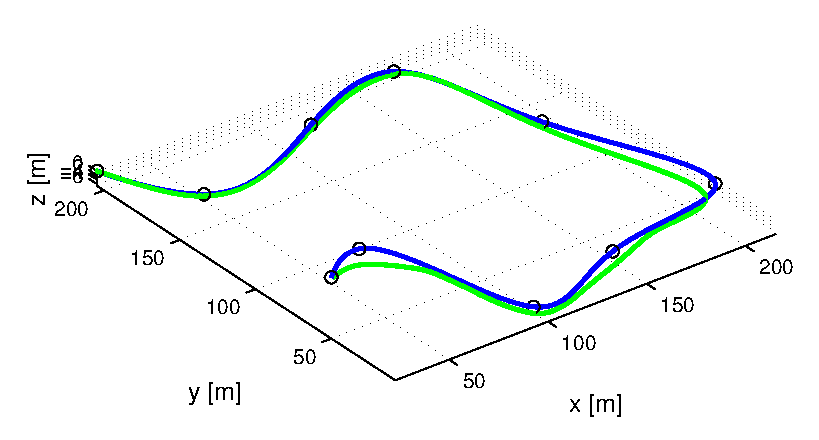
\includegraphics[width = \textwidth]{trackings_wc/figure_3D_road_SplineDegree3_trajectoryFollowing_Disturbance_0}
  \end{minipage}
  \hfill
  \begin{minipage}[t]{0.32\textwidth}
    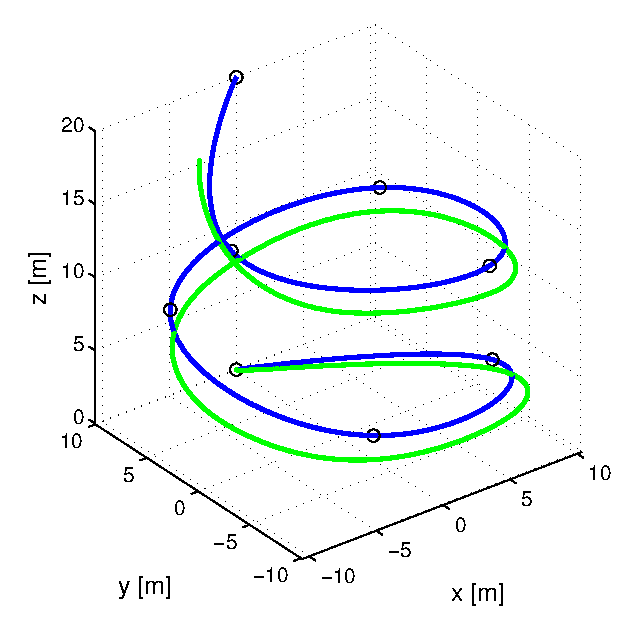
\includegraphics[width = \textwidth]{trackings_wc/figure_3D_helix_SplineDegree3_trajectoryFollowing_Disturbance_0}
  \end{minipage}
  \hfill
  \begin{minipage}[t]{0.32\textwidth}
    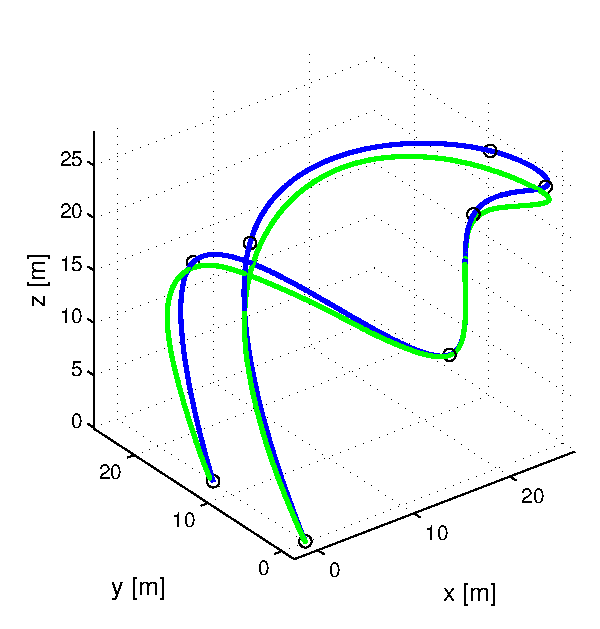
\includegraphics[width = \textwidth]{trackings_wc/figure_3D_agile_SplineDegree3_trajectoryFollowing_Disturbance_0}
  \end{minipage}
  %\caption{BLA tracking }
  \vspace{5pt}
  \begin{minipage}[t]{0.32\textwidth}
    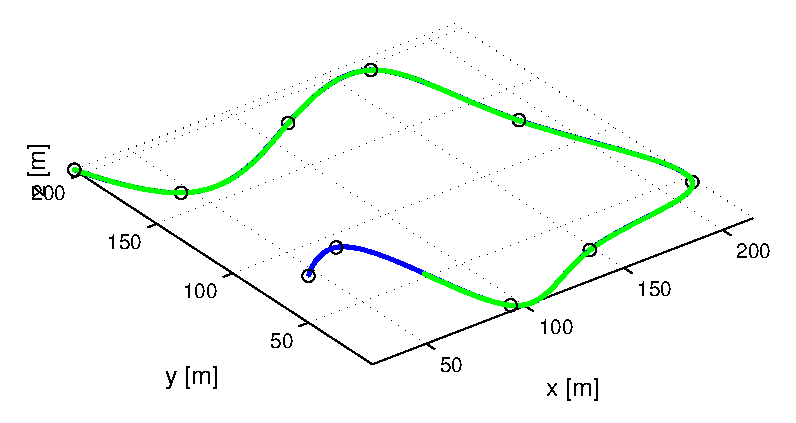
\includegraphics[width = \textwidth]{trackings_wc/figure_3D_road_SplineDegree3_purePursuit_Disturbance_0}
  \end{minipage}
  \hfill
  \begin{minipage}[t]{0.32\textwidth}
    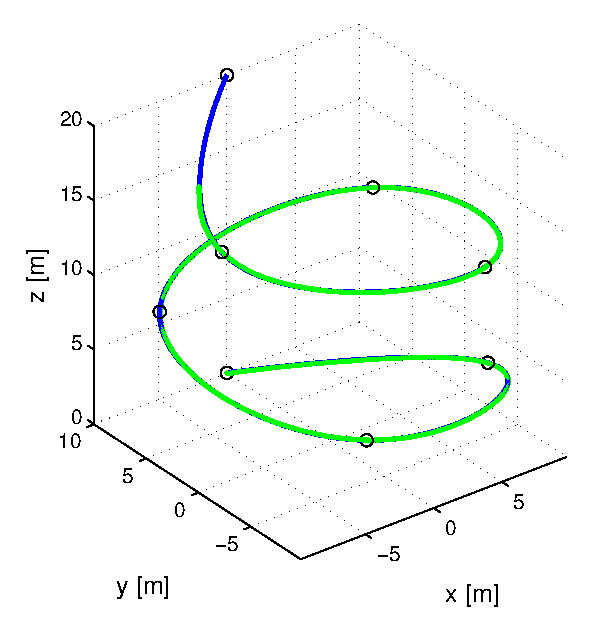
\includegraphics[width = \textwidth]{trackings_wc/figure_3D_helix_SplineDegree3_purePursuit_Disturbance_0}
  \end{minipage}
  \hfill
  \begin{minipage}[t]{0.32\textwidth}
    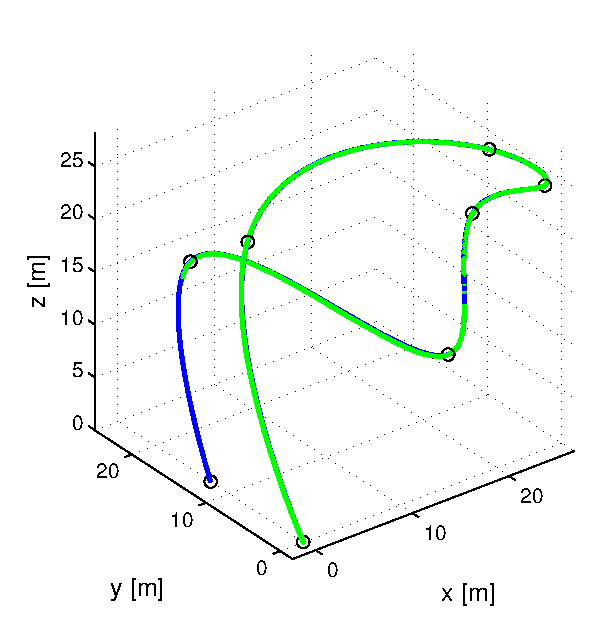
\includegraphics[width = \textwidth]{trackings_wc/figure_3D_agile_SplineDegree3_purePursuit_Disturbance_0}
  \end{minipage}
  %\caption{BLA tracking }
  \vspace{5pt}
  \begin{minipage}[t]{0.32\textwidth}
    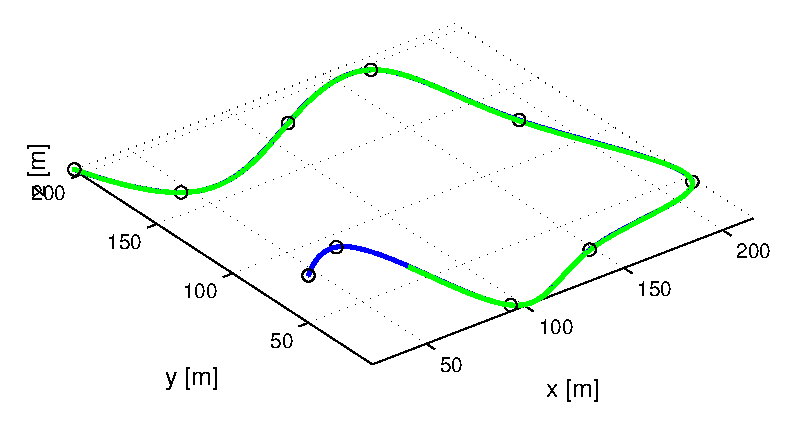
\includegraphics[width = \textwidth]{trackings_wc/figure_3D_road_SplineDegree3_crossTrack_Disturbance_0}
  \end{minipage}
  \hfill
  \begin{minipage}[t]{0.32\textwidth}
    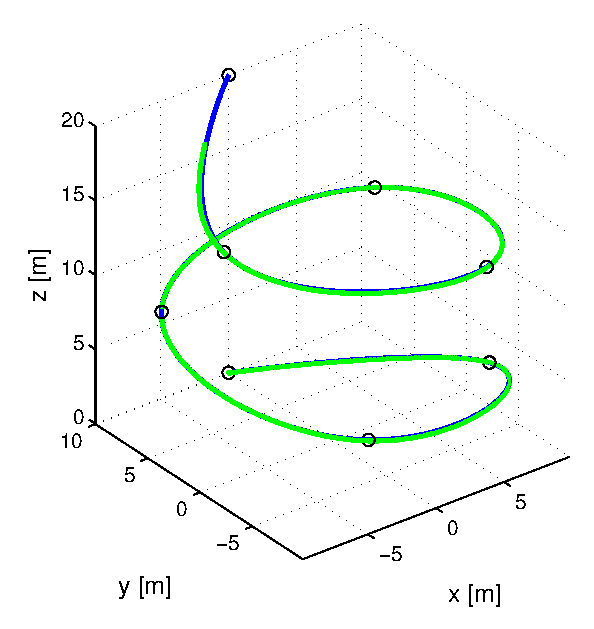
\includegraphics[width = \textwidth]{trackings_wc/figure_3D_helix_SplineDegree3_crossTrack_Disturbance_0}
  \end{minipage}
  \hfill
  \begin{minipage}[t]{0.32\textwidth}
    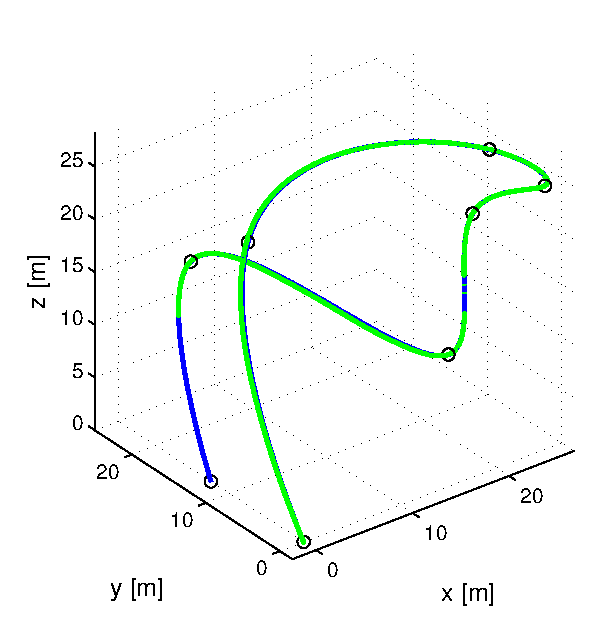
\includegraphics[width = \textwidth]{trackings_wc/figure_3D_agile_SplineDegree3_crossTrack_Disturbance_0}
  \end{minipage}
  \caption{Trajectory tracking with wrong system constraints (+20\%). {\bf Top}: \textit{Trajectory following} control forces the system to reach the end within the given constraints. As trajectory demands too high performance, tracking gets bad. {\bf Center}: \textit{Pure pursuit} control is more robust to the wrong conditioned trajectory and tracking is quite accurate. In comparison to the ideal case it only makes 86-90\% of the track within $T_p$. {\bf Bottom}: \textit{Cross track error} control is accurate and makes 87-93\% of the track within $T_p$.}
  \label{fig:results_model_uncertainties}
\end{figure}

\begin{figure}[h]
  \begin{minipage}[t]{0.48\textwidth}
    \includegraphics[width = \textwidth]{correlation/Control_Correlation_InvDev_Acc_Parametrization_AllCircuits}
  \end{minipage}
  \hfill
  \begin{minipage}[t]{0.48\textwidth}
    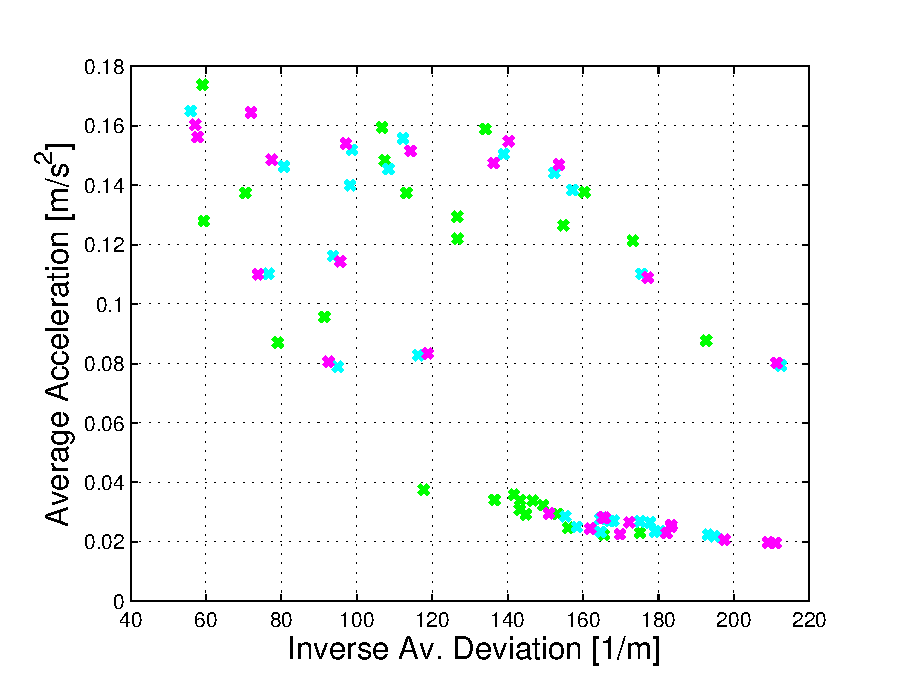
\includegraphics[width = \textwidth]{correlation/Control_Correlation_InvDev_Acc_SplineDegree_AllCircuits}
  \end{minipage}
  \caption{ddddddddddddd}
  \label{fig:correlation_invdev_acc_all_circuits}
\end{figure}

\section{Camparision to system constraints}
Here we show to how the tracking results change if we increase the system's constraints.

\subsection{Increasing the paths curvature}
And here follows a subsection with constraint comparisons of a helix with smaller radius.

 %\cleardoublepage


%\chapter{Nochmals irgendwas}\label{sec:nochirgendwas}

%Bla bla \dots

 %\cleardoublepage
